Este capítulo descreve como o trabalho foi conduzido e como a proposta é avaliada. A Seção~\ref{sec:dsr} apresenta a abordagem de pesquisa. A Seção~\ref{sec:requisitos} define os requisitos que a solução deve atender, antes de qualquer escolha de arquitetura. A Seção~\ref{sec:caso} apresenta o estudo de caso e os dados utilizados, e a Seção~\ref{sec:experimentos}, os experimentos e os seus critérios de aprovação. As Seções~\ref{sec:validacao} e~\ref{sec:reprodutibilidade} tratam, por fim, de como a avaliação evita conferir a solução contra ela mesma e de como pode ser reproduzida.

\section{Abordagem de pesquisa}\label{sec:dsr}

O trabalho segue a pesquisa em ciência do design (\textit{design science research}, DSR), em que o conhecimento resulta da construção e da avaliação de um artefato dirigido a um problema identificado \cite{hevner2004}. O artefato, aqui, é a arquitetura de dados e a sua implementação. As etapas adotadas são as propostas por \citeonline{peffers2007}, e a Tabela~\ref{tab:dsr-etapas} indica onde cada uma é tratada.

\begin{table}[htbp]
    \centering
    \caption{Etapas da pesquisa em ciência do design e a sua localização no trabalho.}
    \label{tab:dsr-etapas}
    \begin{tabularx}{\linewidth}{X l}
        \toprule
        Etapa & Onde é tratada \\
        \midrule
        Identificação do problema e motivação & Capítulo~\ref{chap:introducao} \\
        Definição dos objetivos da solução & Seção~\ref{sec:requisitos} \\
        Projeto e desenvolvimento do artefato & Seções~\ref{sec:visao-geral} a~\ref{sec:implementacao} \\
        Demonstração & Seção~\ref{sec:aplicacao-sbsj} \\
        Avaliação & Seção~\ref{sec:experimentos} e Capítulo~\ref{chap:resultados} \\
        Comunicação & este texto, a biblioteca e o banco extraído \\
        \bottomrule
    \end{tabularx}
    \par\smallskip{\small Fonte: o autor, a partir de \citeonline{peffers2007}.}
\end{table}

A avaliação é feita por falseamento. Cada propriedade da hipótese é traduzida em uma pergunta de resposta sim ou não, com um critério de aprovação fixado antes da execução. Um experimento reprovado refutaria a propriedade correspondente no caso estudado. Um experimento aprovado não a prova em geral, mas mostra que a arquitetura a sustenta nas condições declaradas.

\section{Requisitos do artefato}\label{sec:requisitos}

Os requisitos descrevem um serviço de dados auditável como uma caixa-preta, isto é, pelas perguntas que ele precisa responder, e não pela forma como as responde. Definidos antes da arquitetura, eles evitam que a solução proposta justifique o próprio problema. A Tabela~\ref{tab:requisitos} os resume, e as subseções seguintes os detalham. O Capítulo~\ref{chap:solucao} mostra, depois, o mecanismo que atende a cada um.

\begin{table}[htbp]
    \centering
    \caption{Requisitos de um serviço de dados auditável.}
    \label{tab:requisitos}
    \begin{tabularx}{\linewidth}{l X}
        \toprule
        Requisito & O serviço deve \\
        \midrule
        R1 Origem de cada valor & informar quem afirmou cada valor, por quê e com base em quais premissas \\
        R2 Reconstrução no tempo & reconstruir o conteúdo de qualquer produto em qualquer instante passado \\
        R3 Consistência entre produtos & impedir que dois produtos referentes ao mesmo instante divirjam \\
        R4 Mínimo de informação & guardar apenas o que não pode ser calculado a partir de outros dados \\
        R5 Posição relativa & registrar posições em relação a pontos medidos, de modo que uma nova medição se propague \\
        R6 Estrutura comum e conteúdo flexível & exigir uma forma mínima comum a todos os elementos e aceitar o restante sem esquema fixo \\
        R7 Verificação por terceiro & permitir que quem recebe os dados confira a sua integridade sem confiar em quem os publica \\
        \bottomrule
    \end{tabularx}
    \par\smallskip{\small Fonte: o autor.}
\end{table}

\subsection{R1: origem de cada valor}\label{sec:req-origem}

O serviço deve informar, para cada valor, quem o afirmou, por que motivo e com base em quais premissas. Essa é a pergunta central de uma auditoria e a que as publicações atuais não respondem (Capítulo~\ref{chap:introducao}). Um valor sem autor e sem causa pode estar correto, mas não pode ser auditado.

\subsection{R2: reconstrução no tempo}\label{sec:req-tempo}

O serviço deve reconstruir o conteúdo de qualquer produto em qualquer instante passado, sem depender de que o usuário tenha guardado a edição correspondente. Este trabalho adota um único eixo de tempo, o de transação (Seção~\ref{sec:bitemporal}), por dois motivos. O primeiro é documental. O que se pretende auditar é o que foi oficialmente afirmado em cada instante, e o tempo de transação responde exatamente a isso. O segundo é metodológico. O segundo eixo traz complexidade própria, como a consulta em duas dimensões e o fim de validade calculável apenas na leitura, que exigiria uma avaliação à parte.

O tempo de validade fica, assim, como extensão. Ele importa porque, sem ele, um erro de dado pode passar por erro operacional. Uma sinalização ou uma distância publicadas de forma errada levam os operadores a criar hábitos para compensá-las, e o registro não mostra que a condição real era outra desde o início.

\subsection{R3: consistência entre produtos}\label{sec:req-consistencia}

Dois produtos referentes ao mesmo instante não podem divergir. O PANS-AIM já exige consistência entre os produtos de informação aeronáutica \cite{icao2018pansaim}. O requisito torna essa exigência verificável. Quando dois produtos divergem, deve ser possível identificar se a causa é o instante consultado ou a regra de cálculo aplicada.

\subsection{R4: mínimo de informação}\label{sec:req-minimo}

O serviço deve guardar apenas o que não pode ser calculado a partir de outros dados. Comprimentos, azimutes e distâncias declaradas resultam de posições medidas e de regras normativas (Seção~\ref{sec:distancias}). Guardá-los ao lado das premissas cria duas fontes para a mesma informação, que podem se contradizer.

O SBSJ ilustra esse risco (Figura~\ref{fig:aip-ad212}). Na seção AD~2.12 da AIP, as observações sobre a pista mencionam a cabeceira~34 como deslocada. Na seção AD~2.13, contudo, a LDA da direção~34 é igual à TORA, o que corresponde a um deslocamento nulo. O texto e a tabela não podem estar ambos certos, e a publicação não permite saber qual dos dois prevalece. Quando a LDA é calculada a partir do deslocamento, registrado como premissa, essa contradição deixa de ser possível.

\begin{figure}[htbp]
    \centering
    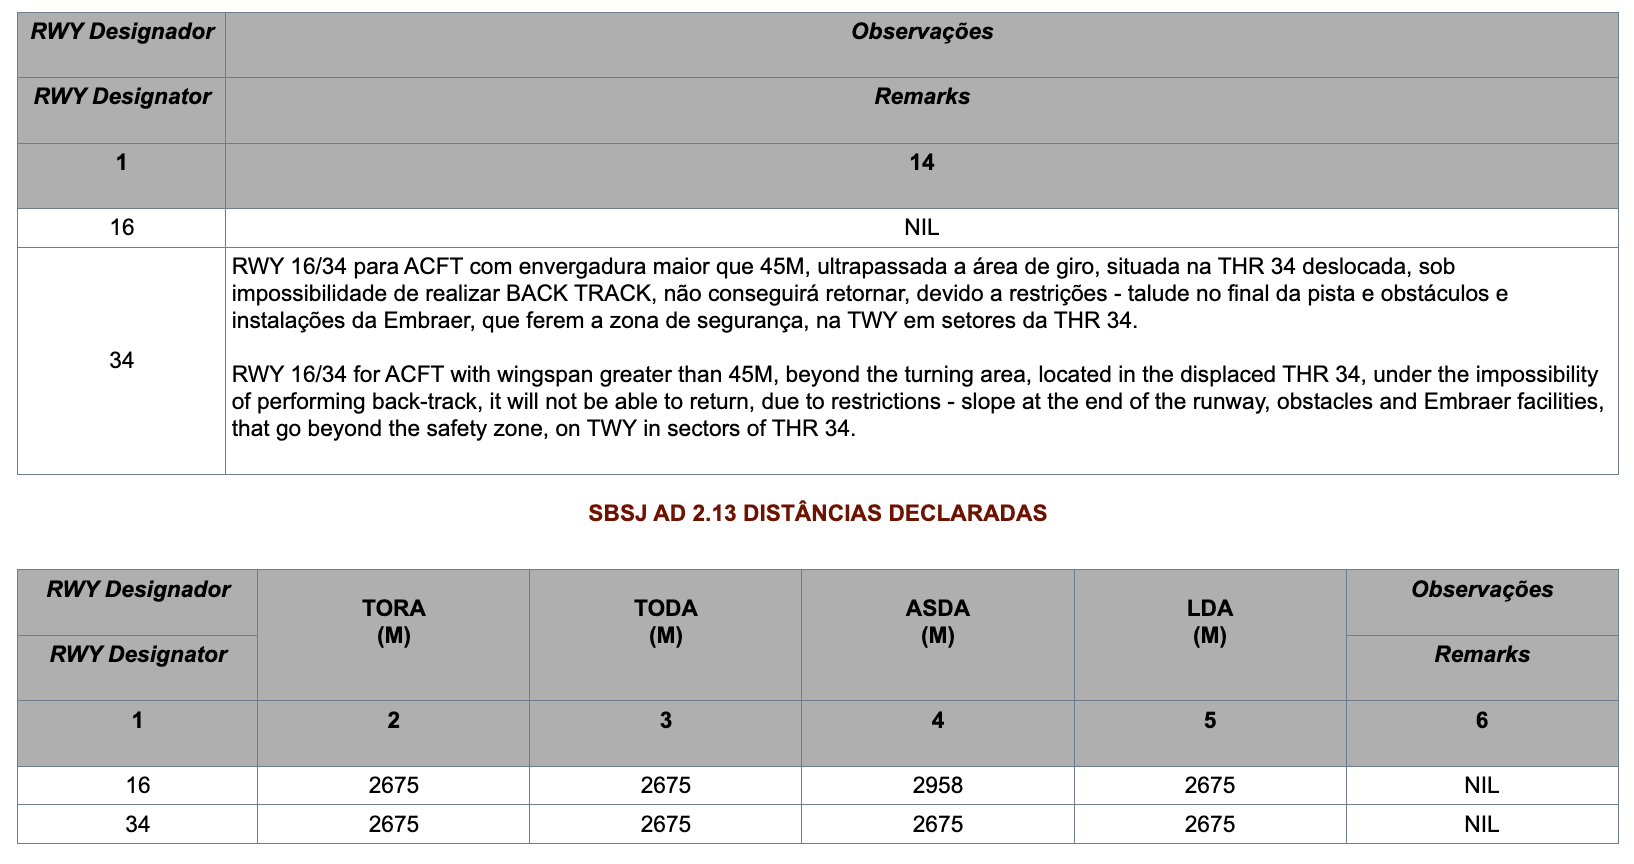
\includegraphics[width=\linewidth]{Figures/aip212.png}
    \caption{Observações da seção AD~2.12 e distâncias declaradas da seção AD~2.13 da AIP do SBSJ.}
    \label{fig:aip-ad212}
    \par\smallskip{\small Fonte: \citeonline{decea2026aip}.}
\end{figure}

\subsection{R5: posição relativa}\label{sec:req-posicao}

As posições devem ser registradas em relação a pontos efetivamente medidos, e não por coordenadas próprias. Uma nova medição de um desses pontos deve, então, propagar-se a todas as posições que dependem dele, sem que nenhuma delas precise ser reescrita. É a propriedade do referenciamento linear (Seção~\ref{sec:iso19148}) aplicada ao lado ar.

\subsection{R6: estrutura comum e conteúdo flexível}\label{sec:req-forma}

Todos os elementos devem compartilhar uma forma mínima, e o restante do conteúdo deve ser livre. A forma mínima é o que permite tratar qualquer elemento da mesma maneira, isto é, a sua identidade, o seu tipo, a sua posição ou relação com outros elementos e as premissas de que dependem os valores derivados. O conteúdo livre acomoda a diversidade entre aeródromos, que nenhum esquema fixo antecipa. Uma informação ausente deve, além disso, distinguir-se de uma informação nula.

\subsection{R7: verificação por terceiro}\label{sec:req-verificacao}

Quem recebe os dados deve poder conferir a sua integridade sem confiar em quem os publica, nem no código de quem os publica. Para isso, a forma de verificação precisa ser pública e simples o bastante para ser reimplementada de forma independente.

\section{Estudo de caso e dados}\label{sec:caso}

O estudo de caso é a pista 16/34 do Aeroporto de São José dos Campos (SBSJ). A escolha se deve a dois fatores. O primeiro é a existência de duas cartas oficiais, de 2022 e de 2026, com valores diferentes para a mesma pista (Figura~\ref{fig:adc-aoc}), o que permite caracterizar a lacuna com dados reais. O segundo é a configuração simples, com uma única pista, que isola as propriedades avaliadas de questões de composição entre vários elementos.

Os dados vêm de três publicações do DECEA:
\begin{itemize}
    \item a AIP, seções AD~2.12 e AD~2.13, com as coordenadas, as elevações e a ondulação geoidal das cabeceiras, a largura da pista, as dimensões da zona de parada e as distâncias declaradas \cite{decea2026aip};
    \item a Carta de Obstáculos de Aeródromo, emenda AIRAC~2213 \cite{decea2022aoc};
    \item a Carta de Aeródromo, emenda AIRAC~2604 \cite{decea2026adc}.
\end{itemize}

Apenas as premissas entram no registro. Os valores que a AIP publica e que podem ser calculados, como o comprimento, os azimutes e as distâncias declaradas, ficam de fora e servem de gabarito. As duas cartas servem apenas ao contraste do E1. A remedição da cabeceira~34 e as restrições temporárias são simuladas, pois não ocorreram no período estudado, e servem para exercitar o ciclo de vida dos elementos.

\section{Experimentos}\label{sec:experimentos}

São seis experimentos, cada um dedicado a uma propriedade da hipótese. O E1 é um contraste. Ele registra os dados na forma em que as publicações chegam ao usuário e verifica o que esse registro permite responder. Os demais usam a arquitetura proposta. A Tabela~\ref{tab:experimentos} apresenta as perguntas e os critérios de aprovação, e a Seção~\ref{sec:procedimentos} descreve como cada experimento é executado.

\begin{table}[htbp]
    \centering
    \caption{Perguntas e critérios de aprovação dos experimentos.}
    \label{tab:experimentos}
    \small
    \begin{tabularx}{\linewidth}{l X X}
        \toprule
        & Pergunta & Critério de aprovação \\
        \midrule
        E1 & O modelo que guarda o valor publicado registra a causa das mudanças entre edições? & contraste: nenhum campo alterado traz causa \\
        E2 & Os valores derivados reproduzem os publicados? A remedição de uma cabeceira obriga a reescrever outro dado? & diferença dentro da margem de cada grandeza; a remedição grava apenas o levantamento e a troca de referencial; diferença ao gabarito geodésico abaixo de 0,5~mm \\
        E3 & O estado em qualquer instante é reconstruído, com autor, motivo e causa de cada mudança? & estados esperados em todos os instantes consultados; derivados de um instante passado idênticos antes e depois da remedição \\
        E4 & Quais alterações feitas diretamente no banco são detectadas, e por qual mecanismo? & alterar, apagar e inserir eventos detectados pela cadeia; reescrita completa detectada pela âncora \\
        E5 & Produtos gerados do mesmo registro divergem? Um terceiro verifica o registro sem a biblioteca? & mesmos valores nos dois produtos; o verificador independente chega à mesma cabeça e aponta o evento alterado \\
        E6 & A leitura pelo tópico equivale à do banco, sem estados intermediários e com o canal adulterado percebido? & mesmas respostas em todos os cortes; nenhum corte dentro de um grupo; recorte com os mesmos derivados; recusa da leitura além do recebido; mesmo \textit{hash} nos seis consumidores; adulteração no meio do tópico interrompe o consumo \\
        \bottomrule
    \end{tabularx}
    \par\smallskip{\small Fonte: o autor.}
\end{table}
% CONFERIR: citar os commits em que as verificações foram registradas antes da execução.

Nenhuma margem foi escolhida livremente. As margens das grandezas publicadas decorrem da precisão com que a AIP publica cada valor e as coordenadas de que ele depende, definida no PANS-AIM \cite{icao2018pansaim}. O comprimento, por exemplo, é publicado ao metro, e as coordenadas das cabeceiras, a 0,01\textquotedbl. O valor calculado pode, então, diferir do publicado em até 0,919~m, sendo 0,5~m do arredondamento ao metro e 0,419~m do efeito do arredondamento das coordenadas. Pelo mesmo raciocínio, resultam $\pm$1,419~m para a ASDA~16, que soma o arredondamento da zona de parada, $\pm$0,014$^\circ$ para os azimutes e $\pm$1,009$^\circ$ para os rumos magnéticos, publicados em graus inteiros, assim como a variação magnética. O Apêndice~\ref{ape:testes} lista as verificações de cada experimento. A comparação com o gabarito geodésico usa a exatidão de 0,5~mm das fórmulas de Vincenty (Seção~\ref{sec:geodesia}). As verificações foram registradas no histórico do repositório de experimentos antes da sua execução \cite{aeroledger_experimentos}.

\section{Verificação interna e comparação externa}\label{sec:validacao}

Uma biblioteca que confere o que ela própria gravou mostra consistência por construção, e não correção. Por isso, a avaliação distingue dois tipos de verificação. A verificação interna confere que a biblioteca devolve o que gravou e que as suas regras são cumpridas. A comparação externa confronta os resultados com referências que não dependem da biblioteca.

Três referências externas são usadas. A primeira são os valores da AIP que não entram no modelo, como o comprimento, os azimutes e as distâncias declaradas, que a arquitetura precisa recalcular. A segunda é um gabarito geodésico, uma implementação das fórmulas de Vincenty escrita separadamente e validada em um caso publicado. A terceira é um verificador independente, escrito apenas a partir da especificação pública da cadeia, sem o código da biblioteca.

\section{Reprodutibilidade}\label{sec:reprodutibilidade}

Os experimentos usam a biblioteca \texttt{aeroledger}, versão 0.6.0 (\textit{commit} \texttt{e93b718}) \cite{aeroledger}, e são executados por um \textit{notebook} mantido em repositório separado \cite{aeroledger_experimentos}. A separação garante que a biblioteca avaliada não contenha código escrito para o experimento. O banco extraído do SBSJ, gerado a partir do mesmo cenário, está publicado como conjunto de dados aberto \cite{aeroledger_dataset} e permite repetir parte da avaliação sem a biblioteca (Seção~\ref{sec:res-banco}).
